
\chapter{Task B}
A* graph search has being implemented on a recursive manner. 
\section{Environment changes}
The main environment will not change from task A. This agent still works on Vertices and Edges. The difference is the way of storing the path. 
The agent in task A stores it in an open list, in the other hand the agent in this case stores the final path in a closed list. The lists 
implemented in this case are bidirectional so the traversal can be done both ways.

\section{Agent description}

\begin{figure}[h]\centering
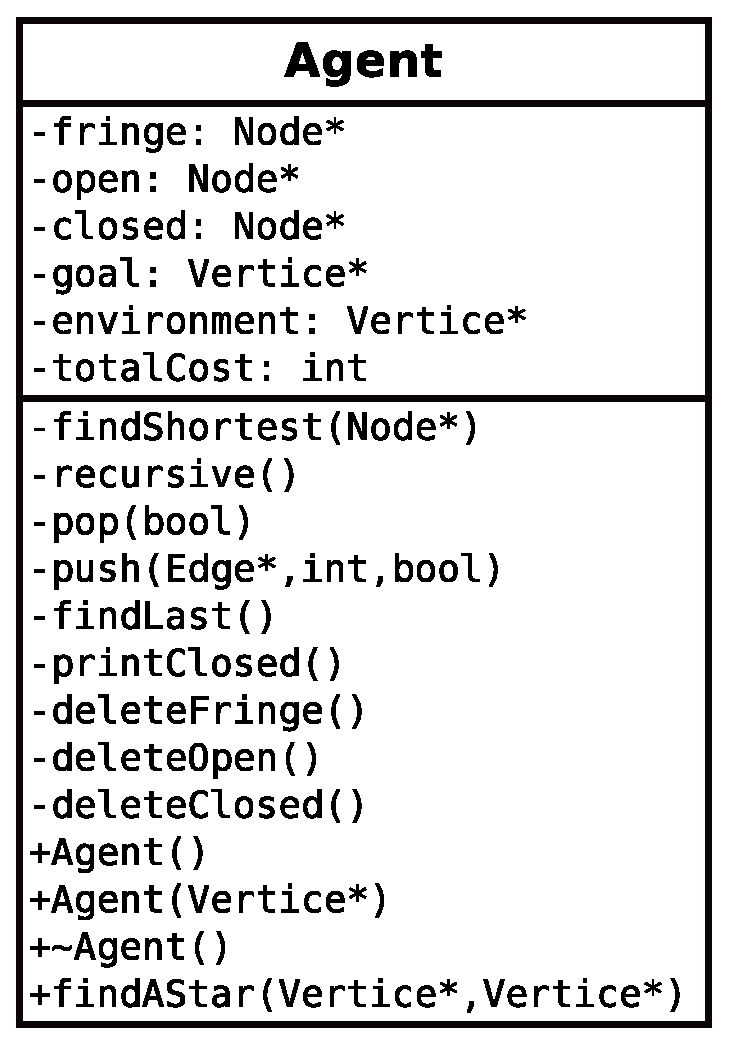
\includegraphics[ width={0.35\textwidth} ]{pictures/uml_agent.eps}
\caption{Description of the A* graph search agent}
\label{fig:uml_agent_graph}
\end{figure}

The agent contains, as shown on the figure \ref{fig:uml_agent_graph}, the following fields:\\
\begin{description}
\item[Fringe:]Open list used in the heuristic, for which we use the shortest path algorithm. The fringe is a pointer to a list of Node, 
a struct described in agent.h and on the picture.
\item[Open:]Open list used in the A* algorithm. It's also a list of Nodes like the fringe.
\item[Closed:]Closed list used to store the final path to the goal. As the Open list and the fringe the closed list is a list of struct Node.
\item[Goal:]Pointer to the goal vertice, is used for compairesons during the hole A* algorithm.
\item[Environment:]Pointer to the beginning of the vertice list. It contains the  environment and is used constantly.
\end{description}

To make the agent be able to execute the A* algorithm we created some helper functions:\\

\begin{description}
\item[findShortest:]Function used to calculate the heuristic value for the A* graph search. Recursivly it stacks values in the Fringe 
and pops from there, until it finds the goal. It gives the total cost of the shortest path in return. It executes recursivly be making a call 
to itself poping the next element in the fringe.
\item[pop:]Funtion that returns the last element in the fringe or the open list, depending on the value of the parameter mode. After 
taking the Node out of the list the list pointer is moved frontwords to the next most probable value.
\item[push:]Function that puts new elements in the lists, it aranges it acording to the cost field int the Node struct. Depending on the 
value provided in the mode parameter the function stores the new element in the fringe or in the open list.
\item[recursive:]Recursive function for calculating the A* graph search algorithm.
\end{description}


\begin{figure}[h]\centering
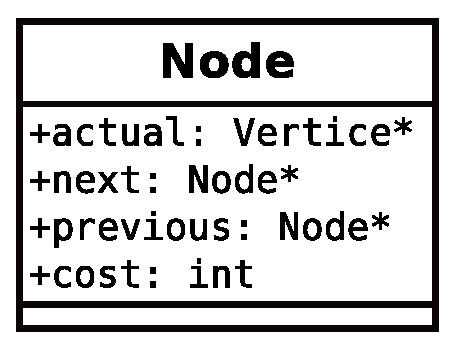
\includegraphics[width=0.35\textwidth]{pictures/uml_node}
\caption{Node structure for list implementation}
\label{fig:node}
\end{figure}


The lists are implemented from the structure Node, see figure \ref{fig:node}. This structure olnly contains the fields:
\begin{description}
\item[Vertice* actual] the vertice pointer that will be used to know the position.
\item[Node* next] next node in the list
\item[Node* previous] is a double linked list, so it has links to the previous nodes.
\item[Int cost] cost of the path to the actual vertice.
\end{description}

\section{A* Star Graph Search algorithm}
The A* graph search implementation is described in this section. It's implemented as a recursive function.\\ 
\begin{description}
\item[The first step] will be to find the heuristic value of the shortest path. This value is calculated with the shortest path algorithm. 
Once we have this value we will use it to make the decissions. We calculate the heuristics this way but the program will be working also 
with other heuristic values.
\item[Second] we add all the edges to the open list making the list longer and will make the program able to move forward.
\item[Third] and last, the program will call itself poping a new element from the open list. If the poped elementis the goal the program 
will finish. 
\end{description}

